\documentclass{standalone}
\usepackage{pgfplots}
\usepackage{pgfplotstable}
\pgfplotsset{compat=1.16}
\usetikzlibrary{matrix,chains,trees,scopes,decorations,arrows.meta,automata,positioning,shadows,3d}



\begin{document}
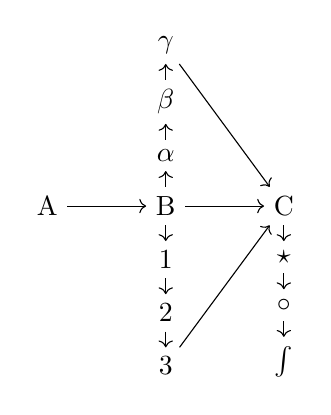
\begin{tikzpicture}[every on chain/.style=join,every join/.style=->,
    node distance=2mm and 1cm]
    { [start chain=trunk]
    \node [on chain] {A};
    \node [on chain] {B};
    { [start branch=numbers going below]
    \node [on chain] {1};
    \node [on chain] {2};
    \node [on chain] {3};
    }
    { [start branch=greek going above]
    \node [on chain] {$\alpha$};
    \node [on chain] {$\beta$};
    \node [on chain] {$\gamma$};
    }
    \node [on chain,join=with trunk/numbers-end,join=with trunk/greek-end] {C};
    { [start branch=symbols going below]
    \node [on chain] {$\star$};
    \node [on chain] {$\circ$};
    \node [on chain] {$\int$};
    }
    }
\end{tikzpicture}
\hspace*{10em}
\begin{tikzpicture}[every on chain/.style=join,every join/.style=->,
    node distance=2mm and 1cm]
    { [start chain=trunk]
    \node [on chain] {A};
    \node [on chain] {B};
    { [start branch=numbers going below] } % just a declaration,
    { [start branch=greek going above] } % we will come back later
    \node [on chain] {C};
    % Now come the branches...
    { [continue branch=numbers]
    \node [on chain] {1};
    \node [on chain] {2};
    }
    { [continue branch=greek]
    \node [on chain] {$\alpha$};
    \node [on chain] {$\beta$};
    }
    }
\end{tikzpicture}
\end{document}